\chapter{Jets data}
\label{ch:jets}
The inclusion of new experimental data is the central element in any global PDFs determination.
New data provide additional constrains on PDFs and allow to get more and more precise results. 
In this Chapter, based on Ref.~\cite{AbdulKhalek:2020jut}, we present a systematic analysis for the inclusion 
of jets cross-sections in a global parton distributions determination.
We will use this specific case to give an example of the general procedure which is usually followed 
when considering new experimental data, using the recent NNLO QCD computations
supplemented by EW corrections to assess the impact of jets and dijets production measurements on the PDFs. 

% 
The choice of the most suitable jest observable to be considered in global PDFs determination and, more in general,
for precision QCD studies presents a number of open theoretical issues, which makes the inclusion of
jest data a particular interesting case.
On one hand, the simplest inclusive observable, 
the single-inclusive jets cross-section~\cite{Ellis:1990ek,Aversa:1988fv}, turns out to be non-unitary.
A possible alternative is offered by the dijets cross-section which however, despite appearing to be 
unitary and especially well suited for PDFs determination~\cite{Giele:1994xd}, at NLO displays a significant scale dependence. 
Thanks to the recent NNLO computation for these observables, this last problem has essentially been settled,
with the scale dependence of dijets cross-section being under control at NNLO.
On the other hand, the single-jet inclusive cross section
shows a scale dependence which is not reduced when going to NNLO~\cite{Currie:2017ctp}, 
showing how the perturbative behaviour, the scale dependence~\cite{Currie:2018xkj} and even the definition~\cite{Cacciari:2019qjx} 
of this observable are non-trivial.  

%
In this study we address these issues from a phenomenological point of view in the context of PDFs determination. 
We study the impact of both single-inclusive
jets and dijets cross-sections in a global parton distributions fit and we
asses which observable leads to better PDFs compatibility with other data, better fit quality,
and more stringent constraint on the parton distributions. 
With this study we aim to provide a guideline for the inclusion of jets observables in a future global fit,
like for example NNPDF4.0.

%
The Chapter is structure as follows. In Sec.~\ref{sec:jets_data} we describe the data included in the analysis,
together with their kinematic coverage; in Sec.~\ref{sec:jets_th} we briefly discuss the main aspects of the theoretical
computation of jets observables, describing the scale choices and the way in which NNLO QCD predictions and EW corrections 
are implemented in the fit; finally in Sec.~\ref{sec:jets_res} we present our results, consisting in a series of global
PDFs fits where different jets observables are included.

\section{Jets data from ATLAS and CMS}
\label{sec:jets_data}
The ATLAS and CMS collaborations have performed a number of measurements of single-inclusive and 
dijets cross sections, with center of mass energies ranging from $\sqrt{s}=2.76$ to $13$ TeV.
In this work we will consider single-inclusive and dijets data at $\sqrt{s}=7$ and $8$ TeV.
%
Whereas recent global PDFs determinations include some jets data, like for instance NNPDF3.1, which includes ATLAS and CMS 
single-inclusive data with $\sqrt{s}=2.76$ and $7$ TeV, this is the first time that the full LHC-Run I jet dataset is being 
considered. In particular dijets data have not been included in any other previous analysis.

%
The specific features of the data considered here are summarized in Table~\ref{tab:input_datasets}:
for each dataset we reported the centre of mass energy $\sqrt{s}$, 
the integrated luminosity $\mathcal{L}$, the jet radius $R$,
the measured differential distribution and the number of datapoints $n_{\text{dat}}$.
The relevant kinematic variables are defined as follows.
For single-inclusive jets we denote as $p_T$ and $y$ the transverse momentum and rapidity.
For dijets, $m_{jj}$ is the invariant dijet mass, $y^*$ and $|y_{\text{max}}|$ are the absolute rapidity difference
and the maximum absolute rapidity of the two leading jets of the event, defined as $y^*=|y_1-y_2|/2$
and $|y_{\text{max}}|= \text{max}\left(|y_1|,|y_2|\right)$ respectively.
Finally, considering the dijets triple differential distribution,
$p_{T,\rm avg} = \left(p_{T_1}+p_{T_2}\right)/2$ is the average transverse momentum of the two leading jets and 
$y_b = |y_1+y_2|/2$ is the boost of the dijets system.

%
The ATLAS 7 TeV data for single-inclusive jet, given as distributions differential in transverse momentum 
$p_T$ and rapidity $y$, cover the kinematic range $100\,\, \text{GeV} \leq p_T \leq 1.992\,\, \text{TeV}$,
$0 \leq |y| \leq 3$, while the ATLAS 8 TeV data cover the same range in rapidity but with an extended transverse momentum
kinematic coverage $70\,\, \text{GeV} \leq p_T \leq 2.5\,\, \text{TeV}$.
In our default fit we include only the central rapidity bin ($y_{jet} \leq 0.5$) of ATLAS 7 TeV, 
for ease of comparison with the NNPDF3.1 analysis of Ref.~\cite{Ball:2017nwa}, where the same choice was adopted due to
the difficulty in achieving a good description of the complete set of rapidity bins using
the default experimental covariance matrix\footnote{In Refs.~\cite{Ball:2017nwa,Nocera:2017zge} this choice was validated,
showing how PDFs determined from each rapidity bin in turn are indistinguishable.}.
The CMS 7 TeV data are available for $100\,\, \text{GeV} \leq p_T \leq 2.0\,\, \text{TeV}$,
$0 \leq |y| \leq 2.5$, and the CMS 8 TeV cover the extended
ranges $74\,\, \text{GeV} \leq p_T \leq 2.5\,\, \text{TeV}$ and $0 \leq |y| \leq 3.0$.

%
Moving to dijets cross-sections, in the case of ATLAS 7 TeV the measurements are double-differential in
$m_{jj}$ and $y^*$, with
$260\,\,\text{GeV}\leq m_{jj} \leq 4.27\,\,\text{TeV}$ and $0 \leq y^* \leq 3.0$, while for CMS 7 TeV
the distributions are differential in  $m_{jj}$ and $|y_{\text{max}}|$, with
$200\,\,\text{GeV}\leq m_{jj} \leq 5\,\,\text{TeV}$ and $0 \leq |y_{\text{max}}| \leq 2.5$.  
Finally the CMS 8 TeV data are triple-differential in $p_{T,\rm avg}$, $y_b$ and $y^*$ with
ranges $133\,\,\text{GeV} \leq p_{T,\rm avg} \leq 1.78\,\,\text{TeV}$ and $0\leq y_b,\,y^* \leq 3$.
Note that ATLAS dijets measurements are currently available at 7 and 13 TeV but not at 8 TeV.

%
In addition to the datasets listed in Table~\ref{tab:input_datasets} ATLAS and CMS have performed
measurements at $\sqrt{s}=13$ TeV for both single-inclusive jet~\cite{Aaboud:2017wsi,Khachatryan:2016wdh}
and dijets~\cite{Aaboud:2017wsi,Sirunyan:2020uoj}. These however have smaller integrated luminosities and for this reason
we do not include these datasets in the analysis. 
%
Finally several measurements for multijets production are also available, with ATLAS providing differential distributions for
three jets cross-sections at 7 TeV~\cite{Aad:2014rma} and four jets cross-sections at 8 TeV~\cite{Aad:2015nda} 
and CMS for three jets at 7 TeV~\cite{CMS:2014mna}.
However theoretical predictions for these observables are currently available only up to NLO, and therefore they will
not be considered here.

%
For all the measurements considered here, the complete set of systematic uncertainties and correlations available from
{\tt HepData} have been used.

%-------------------------------------------------------------------------------
\begin{table}[!t]
    \centering
    \scriptsize
    \renewcommand{\arraystretch}{1.90}
    %-------------------------------------------------------------------------------
\begin{tabularx}{\textwidth}{XXcccccc}
\toprule
  Experiment 
& Measurement   
& $\sqrt{s}$ [TeV]
& $\mathcal{L}$ [fb$^{-1}$] 
& $R$
& Distribution  
& $n_{\rm dat}$ 
& Reference   \\
\midrule
  ATLAS  
& Inclusive jets  
& 7 
& 4.5
& 0.6
& $d^2\sigma/dp_Td|y|$  
& 140  
& \cite{Aad:2014vwa}  \\
  CMS  
& Inclusive jets  
& 7
& 4.5
& 0.7
& $d^2\sigma/dp_Td|y|$  
& 133 
& \cite{Chatrchyan:2012bja}  \\
  ATLAS  
& Inclusive jets  
& 8
& 20.2
& 0.6
& $d^2\sigma/dp_Td|y|$  
& 171  
& \cite{Aaboud:2017dvo}  \\
  CMS  
& Inclusive jets  
& 8 
& 19.7
& 0.7
& $d^2\sigma/dp_Td|y|$  
& 185  
& \cite{Khachatryan:2016mlc}  \\
\midrule
  ATLAS  
& Dijets  
& 7 
& 4.5
& 0.6
& $d^2\sigma/dm_{jj}d|y^{*}|$  
& 90 
& \cite{Aad:2013tea}  \\
  CMS  
& Dijets  
& 7 
& 4.5
& 0.7
& $d^2\sigma/dm_{jj}d|y_{\rm max}|$  
& 54  
& \cite{Chatrchyan:2012bja}  \\
  CMS  
& Dijets  
& 8 
& 19.7
& 0.7
& $d^3\sigma/dp_{T,\rm avg}dy_b dy^{*}$  
& 122  
& \cite{Sirunyan:2017skj}  \\
\bottomrule
\end{tabularx}
%------------------------------------------------------------------------------ 

    \vspace{0.3cm}
    \caption{\small The LHC single-inclusive jet and dijet cross-section data
       that will be used  in this study. For each dataset we indicate the experiment,
       the measurement, the center of mass energy $\sqrt{s}$, the luminosity 
       $\mathcal{L}$, the jet radius $R$, the measured distribution, the number of 
       datapoints $n_{\rm dat}$ and the reference.}
    \label{tab:input_datasets}
\end{table}
%-------------------------------------------------------------------------------
    


\section{Theoretical calculations}
\label{sec:jets_th}
In this section we present the main aspects of the theoretical calculations used to perform
our phenomenological study, discussing scale choices and QCD corrections up to NNLO.
We also discuss EW corrections and the way in which they are combined with QCD predictions for the 
purpose of PDFs determination.

\subsection{Scale choice}
As mentioned at the beginning of this chapter, even when considering NNLO predictions
the single-inclusive jet cross-sections are in general
rather sensible to the choice of central scale.
Three possible choices are given by the individual jet transverse momentum $p_T$, 
the leading jet transverse momentum $p_{T,1}$ and the scalar sum of the transverse momenta of all the partons
in the event 
\begin{align}
    \hat{H}_T = \sum_{i\in\text{partons}} p_{T,i}\,.
\end{align}
Predictions obtained from different scales choices may differ, even at NNLO, by amounts which are comparable to their
scale dependence.
In Ref.~\cite{Currie:2018xkj} the scales $\mu = \hat{H}_T $ and $\mu = 2p_T$ were singled out as optimal ones,
according to a number of criteria, such as perturbative convergence and scale uncertainty as error estimate.
Here we will consider results for $\mu = \hat{H}_T$, which will be compared to those found using $\mu=p_T$,
which was the baseline choice adopted in previous NNPDF dterminations.

%
Turning to dijets observables, also here different scale choices are possible. As mentioned before, at NLO theoretical predictions
computed with different choices differ significantly, however the problem is alleviated at NNLO, with $\mu = m_{jj}$
emerging as preferred choice~\cite{Currie:2017eqf,Currie:2018oxh}, which therefore will be adopted here. 

\subsection{QCD corrections}
As detailed in Chapter~\ref{ch:nnpdf_methodology}, the partonic matrix elements entering a PDFs fit
have to be precomputed in such a way that the numerical convolution with generic input PDFs can be approximated by mean
of interpolation techniques. 
To this purpose we use {\tt NLOJET++}~\cite{Nagy:2001fj} interfaced to {\tt F{\small AST}NLO}~\cite{Wobisch:2011ij}.
The computation is performed using the scale choices described above and is validated against the {\tt NNLOJET} computation.
This fast interpolation grids are then combined with PDF evolution kernel using {\tt APFEL{\small GRID}}~\cite{Bertone:2016lga}
to obtain FK tables, as described in Eq.~\ref{eq:DY_obs}.
However fast interpolation grids to be used as input for {\tt APFEL{\small GRID}} are available only at NLO.
We therefore implement NNLO QCD corrections by supplementing the NLO grids with QCD $K$-factors as detailed in the following.
We computed exact NNLO QCD predictions using {\tt NNLOJET}~\cite{Gehrmann-DeRidder:2019ibf} and we define the 
corresponding $K$-factors as
\begin{align}
    \label{eq:QCD_kfactors}
    K^{\text{QCD}}_{\text{NNLO}} = \frac{\sum_{ij}\hat{\sigma}_{ij}^{\text{NNLO}}\otimes \mathcal{L}_{ij}^{\text{NNLO}}}
    {\sum_{ij}\hat{\sigma}_{ij}^{\text{NLO}}\otimes \mathcal{L}_{ij}^{\text{NNLO}}}\,,
\end{align}
where the sum runs over partonic subchannels, $\hat{\sigma}_{ij}$ are partonic matrix elements and $\mathcal{L}$
the corresponding parton luminosity, computed in both the numerator and denominator using NNPDF3.1 NNLO as a fixed input 
PDF set.
NNLO grids for the relevant cross-sections are then obtained from the corresponding NLO grids through the multiplicative
prescription
\begin{align}
    \label{eq:NNLO_kfactors}
    \frac{d^2\sigma}{dp_T dy}\Bigg|_{NNLO} = \frac{d^2\sigma}{dp_T dy}
    \Bigg|_{\rm NLO_{QCD}} \times K_{\rm NNLO}^{\rm QCD}(p_T,y,\sqrt{s})\, .
\end{align}
The first term on the right-hand side is the output of the NLO computation, given in terms of fast interpolation grids,
while the second term is the bin-by-bin QCD $K$-factors computing according to Eq.~\ref{eq:QCD_kfactors}. 
The result is validated against the full NNLO result from {\tt NNLOJET}. In general QCD $K$-factors might be affected by 
point-to-point fluctuations due to underlying numerical uncertainties affecting the NNLO computation,
therefore they are provided with a Monte Carlo uncertainty, estimated as described in Ref.~\cite{Ridder:2016rzm}.
This uncertainty is added in quadrature to the experimental one when performing the PDFs fit, fully uncorrelated datapoint 
by datapoint.
For illustration purpose, NNLO QCD $K$-factors for the central rapidity bins $0\leq |y| \leq 0.5$
of thevATLAS 7 TeV single-inclusive jet and of the CMS 8 TeV dijet distributions are displayed 
in Fig.~\ref{fig:kfactqcd_werrors} as functions of $p_T$, together with the corresponding Monte Carlo uncertainties.
In both cases the NNLO QCD $K$-factors increase monotonically with $p_T$ from about $5\%$ to about $20\%$ for single-inclusive
jets, and from about $3\%$ to $15\%$ for dijets. 
\begin{figure}[!t]
    \centering
    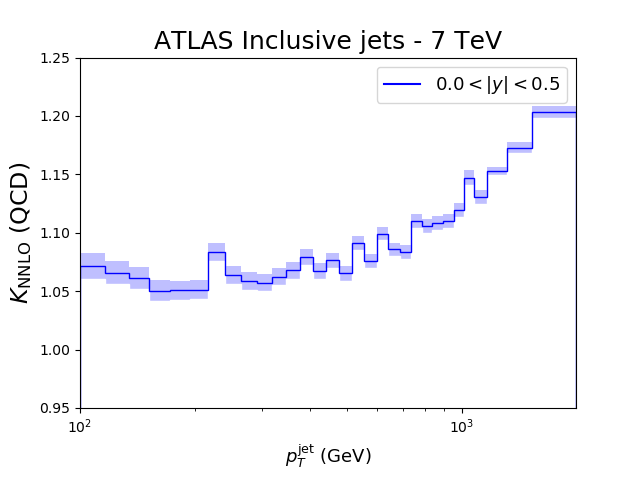
\includegraphics[scale=0.44]{kfactqcd_incljets_atlas7_HTp_R06-rap1-werrors-hist.png}
    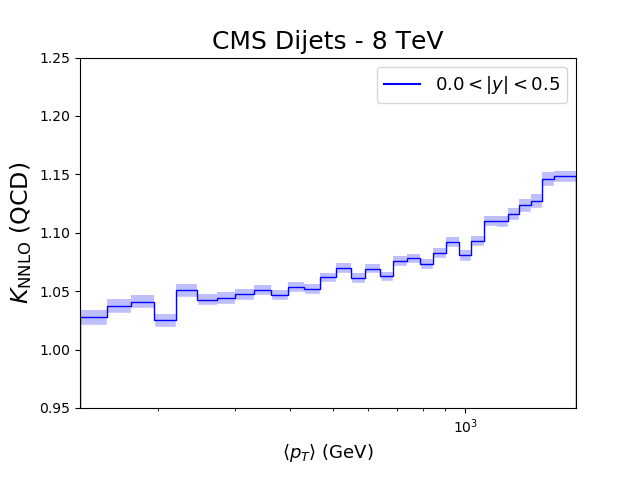
\includegraphics[scale=0.44]{kfactqcd_dijets_cms8_mjj_R07-rap1-werrors-hist.png}
    \caption{The NNLO QCD $K$-factors for the central rapidity bins of the ATLAS 
       7~TeV single-inclusive jets (left) and CMS 8~TeV dijets (right), with
       the Monte Carlo numerical uncertainties shown as filled bands around the 
       central result. Figure from Ref.~\cite{AbdulKhalek:2020jut}.}
\label{fig:kfactqcd_werrors} 
\end{figure}

\subsection{EW corrections}
The EW corrections for all the single-inclusive jet and dijets datasets considered here have been determined 
using the computation of Ref.~\cite{Dittmaier:2012kx}.
These include the $\mathcal{O}\left(\alpha\alpha_s\right)$ and $\mathcal{O}\left(\alpha^2\right)$ tree level contributions 
and the $\mathcal{O}\left(\alpha\alpha_s^2\right)$ weak radiative corrections, where $\alpha$ and $\alpha_s$
denote the weak and strong coupling respectively.
As in the case of NNLO QCD corrections, EW contributions are included by mean of $K$-factor, defined as
\begin{align}
    \label{eq:EW_kfactors}
    K^{\text{EW}} = \frac{\sum_{ij}\hat{\sigma}_{ij}^{\text{LO QCD}+\text{EW}}\otimes \mathcal{L}_{ij}^{\text{NNLO}}}
    {\sum_{ij}\hat{\sigma}_{ij}^{\text{LO QCD}}\otimes \mathcal{L}_{ij}^{\text{NNLO}}}\,,
\end{align}
where the partonic cross sections have been obtained combining the computation of Ref.~\cite{Dittmaier:2012kx} 
with LO QCD results.
Fast interpolation grids accounting for EW corrections can be compute
supplementing Eq.~\ref{eq:NNLO_kfactors} with the EW $K$-factor of Eq.~\ref{eq:EW_kfactors}, getting
\begin{align}
    \label{eq:NNLO_EW_kfactors}
    \frac{d^2\sigma}{dp_T dy}\Bigg|_{NNLO+EW} =\,\,\,\,\,\,\,\, &\frac{d^2\sigma}{dp_T dy} 
    \Bigg|_{\rm NLO_{QCD}} \nonumber\\ &\times K_{\rm NNLO}^{\rm QCD}(p_T,y,\sqrt{s})
    \times K_{\rm NNLO}^{\rm EW}(p_T,y,\sqrt{s})\,.
\end{align}

Electroweak $K$-factors have been computed using a proprietary code, with NNPDF3.1 NNLO PDF set as input.
In Fig.~\ref{fig:kfactewk_dijets7} representative plots are shown for ATLAS 7 TeV single-inclusive jet and CMS 7 TeV dijest,
as functions of $p_T$ (single-inclusive jet) and $m_{jj}$ (dijets), in bins of rapidity $y$
or maximum absolute rapidity $y_{\text{max}}$. In both cases, $K$-factors are close to one for small
values of $p_T$ or $m_{jj}$, they are mostly flat for large values of the rapidity variable while 
they grow with $p_T$ or $m_{jj}$  for the central rapidity bin, reaching values as high as $20\%$.
EW $K$-factors for the other distributions, not displayed here, present similar features.

\begin{figure}[!t]
    \centering
    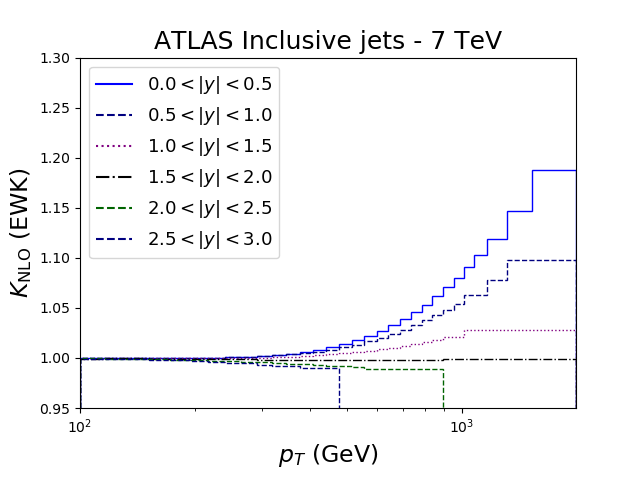
\includegraphics[scale=0.44]{kfactqcd_ewk_incjets_atlas7-hist.png}
    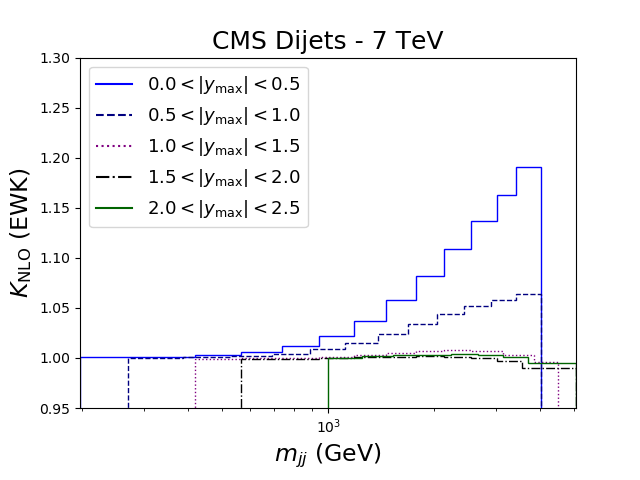
\includegraphics[scale=0.44]{kfactqcd_ewk_dijets_cms7-hist.png}\\
    \caption{The EW $K$-factors, Eq.~\eqref{eq:EW_kfactors}, for the 7 TeV ATLAS and CMS
       single-inclusive (left) and dijet (right)  measurements. For 
       single-inclusive jets the $K$-factors are shown as a function of jet $p_T$ 
       in six different rapidity bins. For dijets they are shown as a function of 
       the dijet invariant mass $m_{jj}$ for different $y_{\rm max}$ bins. Figure from Ref.~\cite{AbdulKhalek:2020jut}.}
    \label{fig:kfactewk_dijets7}
\end{figure}





\section{Results}
\label{sec:jets_res}
In this section we present the main results of our study, consisting in a series of PDF sets
in which the global NNPDF3.1 dataset described in Sec.~\ref{sec:results_nnpdf} has been supplemented with
subsets of the jets and dijets data described in Sec.~\ref{sec:jets_data}.
We consider a series of different scenarios where we vary the jet observable and the input data. 
Specifically we have performed fit including either single-inclusive or dijets data, in each case considering
either the full dataset or the 7 TeV or 8 TeV data only. 
As described in the previous section we use NNLO QCD theoretical computations supplemented by EW corrections, 
with the scale choice $\mu = \hat{H}_T$ for single-inclusive jet and $\mu = m_{jj}$ for dijets.
%Different fits have been produced using 
%theory computations at pure NLO QCD, pure NNLO QCD and NNLO QCD supplemented by EW corrections.
%Finally, for single-inclusive jet data at 7 TeV, we have also produced fits varying the choice of the central scale,
%taking factorization and renormalization scales to be $\mu = \hat{H}_T$ as default and
%producing results for $\mu = p_T$ as well.
%For dijets we always consider $\mu = m_{jj}$. 

%
In Table~\ref{tab:listfits} we report the full list of fits which will be discussed in the following, together 
with an ID that will be used to identify them.
The ID encodes the process used (j for single-inclusive
jets and d for dijets); the data used (a for all, 7 or 8 for the
7~TeV or 8~TeV datasets); 
finally n stands for the perturbative accuracy NNLO QCD and w reminds that EW corrections are included;
Each row of corresponds to a different input datasets, with the fit \#bn representing the baseline, where no jets
data are included. 

%
In all these fits the systematic uncertainties are implemented as fully correlated across bins of different kinematic 
variables, while statistical uncertainties are correlated only across bins of transverse momentum (for jets) or 
invariant mass (for dijets). Following the standard NNPDF methodology, multiplicative uncertainties are 
treated with the $t_0$-method~\cite{Ball:2009qv} and all the fits reported in Table~\ref{tab:listfits} have been iterated once
in order to ensure convergence of preprocessing and $t_0$ method.
The fits have been run using the standard NNPDF methodology described in Sec.~\ref{sec:nnpdf_meth}, employing
the {\tt c++} framework used to produce the NNPDF3.1 PDF set.
All PDF sets discussed contains $N_{\text{rep}}=100$ Monte Carlo replicas, 
and the {\tt ReportEngine} software \cite{zahari_kassabov_2019_2571601} is used 
to analyze results and compute various fit metrics and statistical estimators.  
\begin{table}[!t]
    \renewcommand*{\arraystretch}{1.60}
    \scriptsize
    \centering
    %-------------------------------------------------------------------------------
\begin{tabularx}{\textwidth}{Xlll}
    \toprule
    & NNLO$_{\rm QCD}$+EW
    & NNLO$_{\rm QCD}$
    & NLO$_{\rm QCD}$\\
    \midrule
    baseline (see text)                           &  ---      &  bn     & b    \\
    \midrule
    ATLAS \& CMS jets   7-8~TeV                   & janw      & ---    & ---   \\
    ATLAS \& CMS jets   7~TeV                     & j7nw      & j7n    & j7    \\
    ATLAS \& CMS jets   7~TeV ($\mu=p_T^{\rm jet}$) &  ---      & j7n-pt & j7-pt \\
    ATLAS \& CMS jets   8~TeV                     & j8nw      & j8n    & j8    \\
    \midrule
    ATLAS \& CMS dijets 7-8~TeV                   & danw      & ---    & ---   \\
    ATLAS \& CMS dijets 7~TeV                     & d7nw      & d7n    & d7    \\
    CMS          dijets 8~TeV                     & d8nw      & d8n    & d8    \\
    \bottomrule
    \end{tabularx}
    %-------------------------------------------------------------------------------
    \vspace{0.3cm}
    \caption{The PDF determinations discussed in this study and their
      IDs. Each row corresponds to a different choice of input jet dataset, 
      specified in the first column.
      The ID encodes the process used (j for single-inclusive
      jets and d for dijets); the data used (a for all, 7 or 8 for the
      7~TeV or 8~TeV datasets); the perturbative accuracy (n for QCD NNLO, w for EW corrections).
      In this and subsequent tables and plots ``jets'' is short for single-inclusive jets.}
    \label{tab:listfits}
\end{table}

\begin{table}[t]
    \renewcommand*{\arraystretch}{1.60}
    \scriptsize
    \centering
    %-------------------------------------------------------------------------------
\begin{tabularx}{\textwidth}{Xrcccc}
    \toprule
     Dataset                    & $n_{\rm dat}$ &    bn   &  janw  &      j7nw  &      j8nw  \\
    \midrule
     DIS NC                     &       2103  &    1.17  &  1.18  &    1.17  &    1.18  \\
     DIS CC                     &        989  &    1.10  &  1.11  &    1.10  &    1.11  \\
     Drell-Yan                  &        577  &    1.33  &  1.30  &    1.31  &    1.31  \\
     $Z$ $p_T$                  &        120  &    1.01  &  1.02  &    1.02  &    1.03  \\
     Top pair                   &         24  &    1.05  &  1.25  &    1.02  &    1.24  \\
     Jets (all)                 &        520  &  [2.60] &  1.88  &  [2.53] &  [1.89] \\
     \ \ Jets (fitted)          &             &    ---   &  1.88  &    1.12    &  2.20  \\
     \ \ ATLAS 7 TeV            &         31  &  [1.87] &  1.59  &   1.15   & [1.62] \\
     \ \ ATLAS 8 TeV            &        171  &  [5.01] &  3.22  &  [4.58]   &  3.25  \\
     \ \ CMS   7 TeV            &        133  &  [1.06] &  1.09  &    1.11   & [1.14] \\
     \ \ CMS   8 TeV            &        185  &  [1.59] &  1.25  &  [1.80]   &  1.23  \\
     Dijets (all)               &        266  &  [3.07] & [2.10] &  [2.56]  & [2.22] \\
     \ \ Dijets (fitted)        &             &    ---   &  ---   &    ---      &  ---   \\
     \ \ ATLAS 7 TeV            &         90  &  [2.47] & [1.95] &  [1.97]  & [2.01] \\
     \ \ CMS   7 TeV            &         54  &  [2.40] & [2.08] &  [2.12]  & [2.15] \\
     \ \ CMS   8 TeV            &        122  &  [3.81] & [2.21] &  [3.20]  & [2.39] \\
    \midrule
     Total                      &             &   1.18   &  1.28  &   1.17    &  1.27  \\
    \bottomrule
    \end{tabularx}
    %-------------------------------------------------------------------------------
    \vspace{0.3cm}
    \caption{The $\chi^2$ per datapoint for all fits of
      Table~\ref{tab:listfits} including single-inclusive jet data, with default settings.
      Results are shown
      for all datasets, aggregated by process type. For jets data, results are
      shown both for the sets included in each fit, and also for those not
      included, enclosed in square brackets. Combined results are also shown
      for all single-inclusive jet and for all dijet data, both for
      the full set, and for those included in each fit.
      The number of datapoints in each
      dataset is also shown.}
    \label{tab:chi2s}
\end{table}

\begin{table}[t]
    \renewcommand*{\arraystretch}{1.60}
    \scriptsize
    \centering
    %-------------------------------------------------------------------------------
\begin{tabularx}{\textwidth}{Xrcccc}
    \toprule
     Dataset                    & $n_{\rm dat}$ &   bn   &  danw  &  d7nw  &  d8nw  \\
    \midrule
     DIS NC                     &       2103  &  1.17  &  1.18  &  1.17  &  1.18  \\
     DIS CC                     &        989  &  1.10  &  1.12  &  1.09  &  1.12  \\
     Drell-Yan                  &        577  &  1.33  &  1.29  &  1.32  &  1.28  \\
     $Z$ $p_T$                  &        120  &  1.01  &  1.07  &  1.03  &  1.08  \\
     Top pair                   &         24  &  1.05  &  1.14  &  1.04  &  1.26  \\
     Jets (all)                 &        520  & [2.60] & [2.06] & [2.70] & [2.14] \\
     \ \ Jets (fitted)          &             &  ---   &  ---   &  ---   &  ---   \\
     \ \ ATLAS 7 TeV            &         31  & [1.87] & [1.63] & [1.74] & [1.61] \\
     \ \ ATLAS 8 TeV            &        171  & [5.01] & [3.36] & [4.65] & [3.55] \\
     \ \ CMS   7 TeV            &        133  & [1.06] & [1.06] & [1.14] & [1.07] \\
     \ \ CMS   8 TeV            &        185  & [1.59] & [1.64] & [2.17] & [1.68] \\
     Dijets (all)               &        266  & [3.07] &  1.65  & [2.16] & [1.71] \\
     \ \ Dijets (fitted)        &             &  ---   &  1.65  &  1.72  &  1.68  \\
     \ \ ATLAS 7 TeV            &         90  & [2.47] &  1.76  &  1.78  & [1.78] \\
     \ \ CMS   7 TeV            &         54  & [2.40] &  1.60  &  1.63  & [1.66] \\
     \ \ CMS   8 TeV            &        122  & [3.81] &  1.58  & [2.67] &  1.68  \\
    \midrule
     Total                      &             &  1.18  &  1.22  &  1.19  &  1.20  \\
    \bottomrule
    \end{tabularx}
    %-------------------------------------------------------------------------------
    \vspace{0.3cm}
    \caption{Same as Table~\ref{tab:chi2s}, but now for dijets. The
      baseline is repeated for ease of reference.}
    \label{tab:chi2sD}
\end{table}


%
In Table~\ref{tab:chi2s} we report the $\chi^2$ values for all the fits with single-inclusive jet data listed in 
Table~\ref{tab:listfits}, while in Table~\ref{tab:chi2sD} we report values for dijets fits.
In both cases values reported in square brackets are referred to points not included in the corresponding fit. 
We show the $\chi^2$ values for all the data in the global dataset, grouped by process type 
(DIS NC, DIS CC, Drell-Yan, $Z\,\,p_T$, top pair) and for all jest data, both those included in the fit 
and those which are not.
 

\subsection{Single-inclusive jets}
\label{sec:single_jet}
We first analyze results concerning the inclusion of single-inclusive jet data only.
In Fig.~\ref{fig:jet_data_total} (left) we show the distances between the central values of the fits \#bn and \#janw, 
namely the baseline not including any jets data and the one including all single-inclusive jet cross-sections.
From the distances plot it is clear how single-inclusive jet data have an impact only on the gluon distribution,
the most affected regions being $x\simeq 0.05$, $0.1\lesssim x \lesssim 0.2$, and
$0.3\lesssim x\lesssim 0.5$, with the gluon PDF changing by up to almost one sigma. 
Looking at the PDFs plot in the right panel of Fig.~\ref{fig:jet_data_total} we notice how at small-$x$ 
the gluon distribution is suppressed by about $2\%$ and enhanced by about $4\%$ in the large-$x$ region.
%
Looking at the $\chi^2$ values in Table~\ref{tab:chi2s}, individual jet datasets show a $\chi^2$ per datapoint 
of order one, with the only exception for 8 TeV ATLAS data, for which we get $\chi^2 = 3.22$.
It is interesting to note that the inclusion of singe-inclusive jet data leads also to an improvement 
of the description of dijets data, for which \#janw shows better $\chi^2$ than the baseline fit \#bn.
%   
We observe a mild deterioration of the $\chi^2$ for top pair processes, with a value of 1.25 to be compared to
1.05 of the baseline. A closer investigation shows that this comes from the deterioration in the description 
of the ATLAS top pair rapidity distributions, whose $\chi^2$ per datapoint increases from 1.22 to 2.01.

\begin{figure}[!t]
    \centering
    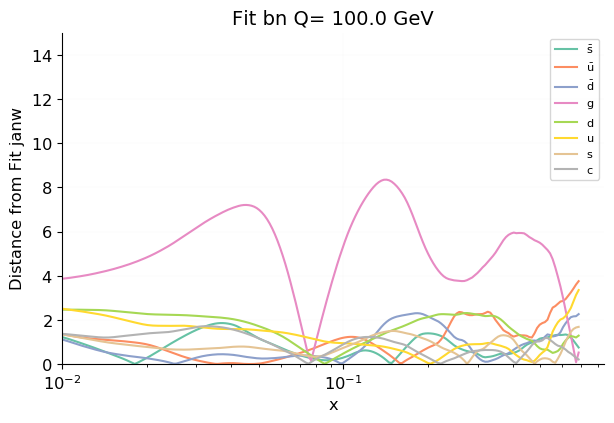
\includegraphics[scale=0.45]{distance_janw_bn}
    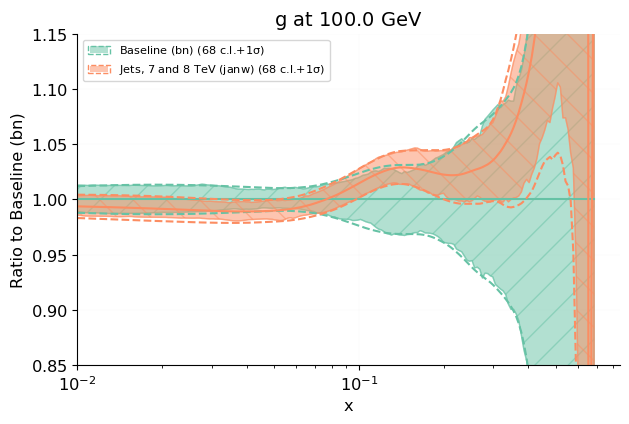
\includegraphics[scale=0.45]{jet_data_1}\\
    \caption{ Comparison between the baseline fit with no jet data  (\#bn)
      and the fit with all single-inclusive jet data included (\#janw).
      The distance between all PDFs
      (left) and the ratio of the gluon PDF to the baseline (right) are shown at the scale
      $Q=100$~GeV. The shaded band is the 68\% confidence interval,
      while the dashed lines are the edge of one sigma interval.}
    \label{fig:jet_data_total}
\end{figure}

%
We can asses the impact of different datasets considering fits with 7 TeV or 8 TeV data only, denoted as \#j7nw and \#j8nw
respectively. From Table~\ref{tab:chi2s} we see how the unsatisfactory description of the 8 TeV ATLAS data persists even when 
no 7 TeV data are included in the analysis, suggesting a possible problem with the dataset itself rather than 
the presence of internal tension with the 7 TeV measurements.
A significant difference between 7 and 8 TeV datasets is that for the former only the central rapidity bin is considered,
as mentioned in Sec.~\ref{sec:jets_data}, while for the latter all the rapidity bins are included.
This suggests that the 8 TeV data may also be affected by similar issues in the treatment of correlations 
between rapidity bins as those observed in the 7 TeV case in Refs.~\cite{Ball:2017nwa}. This problem is addressed
in App.~\ref{app:jets} where we will see that this is indeed the case.
%
Looking at the $\chi^2$ for top pair processes, we note how its deterioration with respect to the baseline value comes
entirely from the inclusion of 8 TeV data.
In Fig.~\ref{fig:jet_data_partial}
we plot the gluon PDF and the corresponding error: for both the 7 TeV and 8 TeV data, the results show 
an enhancement of the central gluon PDF at large-$x$ and a suppression at small-$x$, and a general reduction in the 
PDF uncertainty, which is more marked in the case of the 8 TeV data. 
In general, results obtained including 8 TeV data only are very close to those of the fit \#janw, showing
how 8 TeV datasets provide the dominant contribution, driving the impact of single-inclusive jet data on the final PDFs.

\begin{figure}[!t]
    \centering
    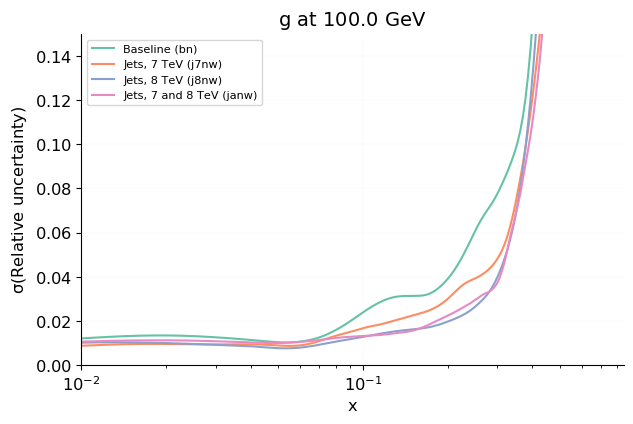
\includegraphics[scale=0.44]{jet_data_3}
    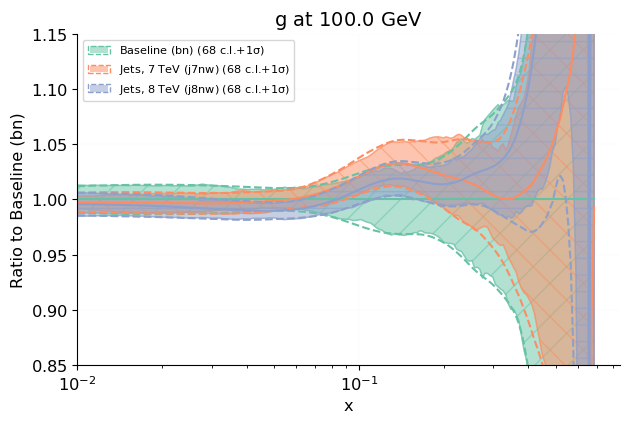
\includegraphics[scale=0.44]{jet_data_2}
    \caption{ Comparison between the baseline fit with no jet data
      (\#bn), and the fits with only 7~TeV (\#j7nw) or only 8~TeV (\#j8nw)
      jet data included. The relative uncertainty on the gluon PDF (left)
      and the ratio of the gluon PDF to the baseline (right) are shown at
      $Q=100$ GeV. All results are shown as ratios to the baseline.}
    \label{fig:jet_data_partial}
\end{figure}

\subsection{Dijets}
We now turn to PDFs in which dijets data rather than single-inclusive jet data have been included.
As done for the single-inclusive jet data, we start comparing the baseline \#bn, where no jets data are considered,
to \#danw, in which all dijets data are included using NNLO QCD computations with EW corrections.
From Table~\ref{tab:chi2sD} we see how all the dijets datasets are fairly well described, with $\chi^2$ values for datapoint
around $1.6$ for each individual dataset. Also, the inclusion of dijets data leads to an improvement in the description
of single-inclusive jet data, consistently with what observed in Sec.~\ref{sec:single_jet}, where 
we notice how the inclusion of single-inclusive jet data leads to a better description of dijets data as well.
These features suggest that single-inclusive and dijet data have a similar impact on PDFs, and show consistency
between data for these two observables. 
%
Also, unlike the case of single-inclusive jet data, no tension is observed between dijets data and the baseline dataset,
whose $\chi^2$ is left almost unchanged.
\begin{figure}[!t]
    \centering
    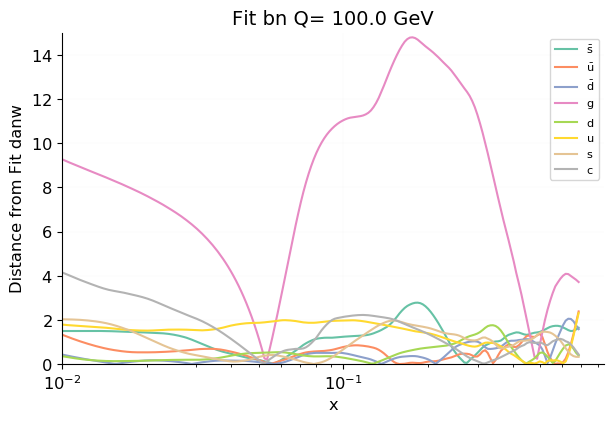
\includegraphics[scale=0.44]{distance_danw_bn}
    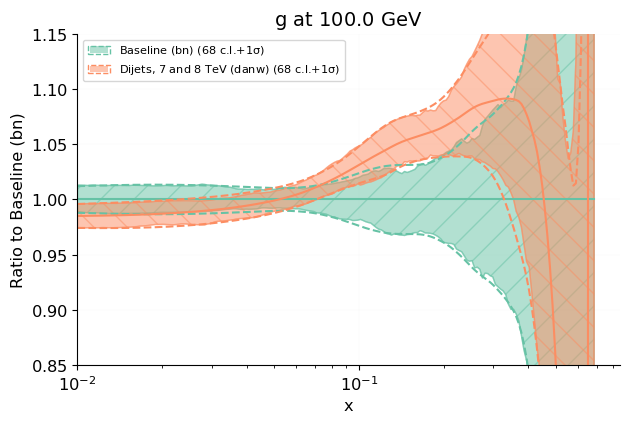
\includegraphics[scale=0.44]{dijet_data_1}\\
    \caption{Same as Fig.~\ref{fig:jet_data_total}, but now for dijets.}
    \label{fig:dijet_data_total}
\end{figure}

%
In the left panel of Fig.~\ref{fig:dijet_data_total} we show the distances between fits \#bn and \#danw: again only
the gluon PDF is affected by the inclusion of the jets data, with the regions $x\simeq 0.01$ and $0.06\lesssim x \lesssim 0.4$
being the ones showing the largest effects.
Looking at the gluon PDF plot in the right panel of Fig.~\ref{fig:dijet_data_total}, we observe a suppression in the former region
by about $2\%$, corresponding to a down shift of the central value by about one sigma, and an enhancement by about $10\%$
in the latter, around $x\sim 0.3$, corresponding to an up shift of the central value by more than one sigma.
%
These features are qualitatively similar to those observed in Sec.~\ref{sec:single_jet} upon inclusion of single-inclusive jet
data, but somewhat more pronounced.    

%
We can study the relative impact of different datasets by studying results for the fits \#j7nw and \#j8nw, where 
either 7 TeV or 8 TeV data only are included.
By inspection of Fig.~\ref{fig:dijet_data_partial}, where we plot the gluon PDF and the corresponding error,
we see how the impact of the two datasets 
on the gluon error and central value is qualitatively the same, and therefore qualitatively equivalent to the one of the 
full dijets dataset, with the 8 TeV data having a stronger impact.
From Table~\ref{tab:chi2sD} we observe how the fit quality is equally good for the two fits.
However the fit including 8 TeV data leads to a similar description of all the dijets data, including those which are
not included in either fits, to the one given by \#danw, where all dijets data are included.
So once again we conclude that the 8 TeV data provide the dominant contribution.
    %-------------------------------------------------------------------------------
    \begin{figure}[!t]
    \centering
    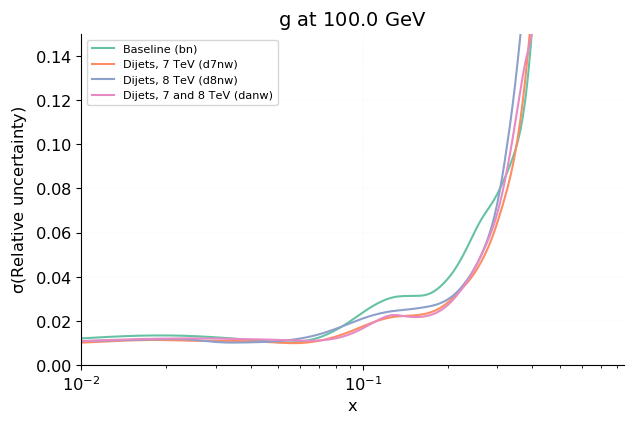
\includegraphics[scale=0.44]{dijet_data_3}
    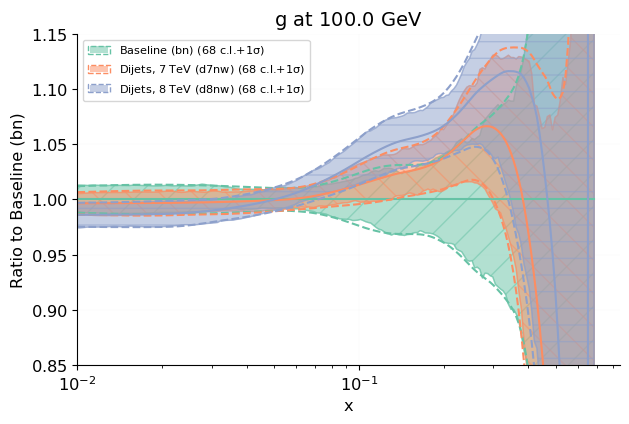
\includegraphics[scale=0.44]{dijet_data_2}
    \caption{Same as Fig.~\ref{fig:jet_data_partial}, but now for dijets.}
    \label{fig:dijet_data_partial}
\end{figure}

\subsection{Single-inclusive jets vs. dijets}
Having assessed the impact on PDFs of jet and dijets datasets separately, we now compare results.

%
The effect on PDFs of the inclusion of jet and dijets in the NNPDF3.1 global dataset is qualitatively the same:
they only affect the gluon, by leading to an enhancement of its central value in the region
$0.1\lesssim x \lesssim 0.4$, and to a  
suppression in the region $0.01\lesssim x \lesssim 0.1$. The suppression
is by about  1\%, while the enhancement at the peak, localized at  $x\simeq 0.3$, is  by about 2.5\%
for single-inclusive jets, but stronger, by about 7.5\% for dijets.
These features are clearly visible in Fig.~\ref{fig:jet_dijet_1} (right), where the gluon PDF is plotted
for the fits \#janw (single-inclusive jet only), \#danw (dijets only) and the baseline \#bn (no jets data).

%
As for the gluon PDF uncertainty, from the left panel of Fig.~\ref{fig:jet_dijet_1} it is clear how
the inclusion of either single-inclusive jet or dijets leads to a reduction of the error, with a stronger
reduction observed in the case of single-inclusive jets. In this respect it should be observed that
ATLAS dijet measurements are not yet available at 8 TeV, while single-inclusive jet measurements are available both from
ATLAS and CMS. The constraining power of dijets datasets is therefore more limited.

%
As for compatibility with the global NNPDF3.1 datasets, the inclusion of jets data does not lead to a deterioration
of the description of the rest of the data in comparison to the baseline fit, as we can see looking at the $\chi^2$
values reported in Tables~\ref{tab:chi2s},~\ref{tab:chi2sD}.
The only exception is the ATLAS top rapidity distribution, which, as mentioned before,
seems to be in tension with the 8 TeV single-inclusive jet data.

%
Concerning fit quality, the quality of the two fits \#janw and \#danw to the corresponding jets data is comparable,
though slightly better for the latter ($\chi^2=1.65$ vs. $\chi^2=1.88$). Also, the quality of the fit to dijets 
when single-inclusive jets are fitted and conversely are almost identical ($\chi^2=2.10$ for dijets when fitting
single-inclusive jets vs. $\chi^2=2.06$ for single-inclusive jets when fitting dijets) and, as observed before,
better then what we get for the baseline.
This confirms full consistency between the two datasets, with a marginal preference for dijets.

%
Finally we note how the fit including dijets data is somewhat more internally consistent than the one including
single-inclusive jets: the $\chi^2$ per datapoint is slightly better (1.22 vs. 1.28) and the $\chi^2$ for individual
dataset is generally better, in particular for top production data.

\begin{figure}[!t]
    \centering
    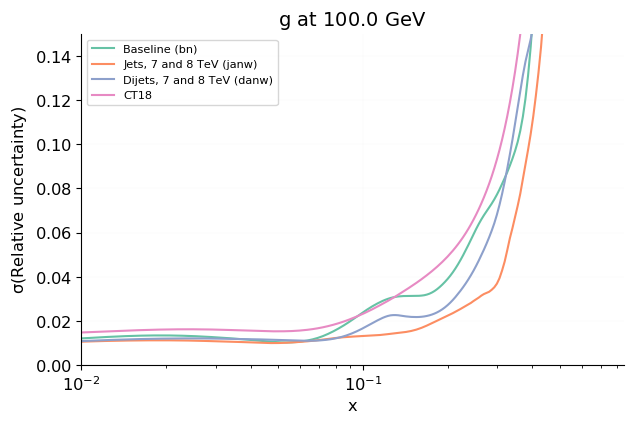
\includegraphics[scale=0.44]{jet_dijet_2}
    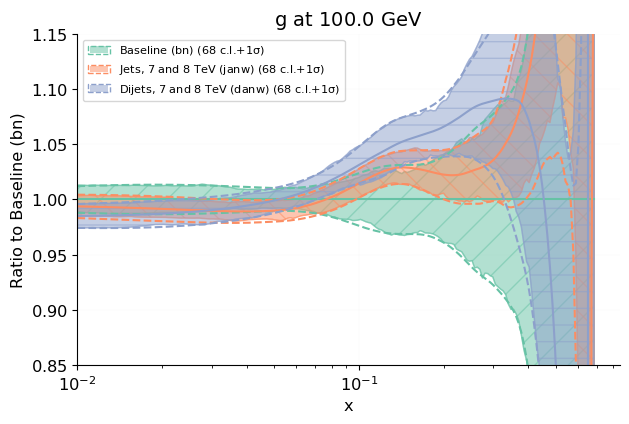
\includegraphics[scale=0.44]{jet_dijet_1}\\
    \caption{Same as Fig.~\ref{fig:jet_data_total}, but now comparing the
      fits with  all single-inclusive jet data (\#janw), and that with all
      dijet data (\#danw).
      In the gluon comparison (right) results are
      displayed as a ratio to the baseline with no jet data included (also
      shown for reference).}
    \label{fig:jet_dijet_1}
\end{figure}

%
To sum up, in this chapter we have presented a phenomenological investigation of inclusive jet
production measurements at LHC in the context of global PDFs determination, exploiting recent NNLO QCD 
theoretical calculations supplemented by EW corrections,
and studying for the first time the impact of the inclusive dijets observables.
We have found full consistency between the impact on parton distributions of dijets and single-inclusive jet data,
thus establishing the viability of the dijets observable in constraining PDFs.
In a comparative assessment of single-inclusive jets vs. dijets we have found how, given the currently available data,
the latter has a more marked impact on the central value of the gluon, 
while the former leads to a more significant reduction of the PDF error. We have also shown evidence of some tension
between some single-inclusive jet datasets and the rest of the global dataset, which might be explained by the less stable
perturbative behaviour of this observable.
Finally we have shown how, both for single-inclusive jets and dijets, the more recent 8 TeV data have a more significant
impact than the previous 7 TeV data. We therefore expect that the future availability of more precise measurements
from LHC Run-II at 13 TeV data will improve further our knowledge of the gluon PDF.   